\documentclass[12pt]{article}

\usepackage{sbc-template}

\usepackage{graphicx,url}

\usepackage{listings}
\usepackage{xcolor}
\lstset { %
    language=C,
    %backgroundcolor=\color{black!5}, % set backgroundcolor
    basicstyle=\tiny,% basic font setting
}


\usepackage[brazil]{babel}   
%\usepackage[latin1]{inputenc}  
\usepackage[utf8]{inputenc}  
% UTF-8 encoding is recommended by ShareLaTex
\usepackage{multicol}
\usepackage[none]{hyphenat}
\newenvironment{Figure}
  {\par\medskip\noindent\minipage{\linewidth}}
  {\endminipage\par\medskip}     
\sloppy

\title{Relatório de Entrega de Trabalho \\
       %Disciplina de programação Paralela (PP) \\ Prof. César De Rose \\
       Exercício 2}

\author{Leonardo G. Carvalho(pp12816), Matheus S. Redecker(pp12819)}


%\address{Pontifícia Universidade Católica do Rio Grande do Sul - PUCRS
%  \email{  \{leonardo.gubert\}\{matheus.redecker\} @acad.pucrs.br}
%}


\begin{document} 

\maketitle

{\small
\begin{multicols}{2}
\section{Introdução}
O objetivo deste trabalho é implementar, utilizando a biblioteca MPI, uma versão paralela de um programa que ordena um vetor utilizando o modelo divisão e conquista e um algoritmo \textit{Bubble Sort}. A modelagem do problema foi pensada em dado um delta, o nodo que recebe o vetor e decide se deve ordenar(conquistar) ou dividir na metade e repassar para os nodos filhos. Para que isso aconteça é preciso ter um controle no número de nodos e no valor de delta, na modelagem apenas os nodos folha realizam a ordenação e os nodos superiores realizam a junção dos vetores ordenados.

\section{Implementação}
Para resolver esse problema o programa foi dividido em duas partes: A primeira parte é a de inicialização para o nodo raiz e a de recebimento para os demais nodos, já a segunda parte é responsável pela escolha se o nodo deve conquistar(ordenar) ou dividir(dividir o vetor em dois e mandar para os dois filhos). Na primeira parte, se o nodo é o processo 0 (raiz) ele deve iniciar o vetor e preenche-lo, se forem os demais processos, devem esperar receber a sua parte do vetor que será enviada pelo nodo pai. Na segunda parte é onde o nodo decide se irá dividir ou conquistar, se o tamanho do vetor recebido for menor ou igual que o delta ele conquista(ordena), se não for ele deve enviar para os seus dois filhos metade do vetor que ele tem. Após ter enviado o processo espera receber os vetores de volta para então realizar o processo de \textit{interleaving} que pega dois vetores ordenados e devolve um vetor apenas, dessa forma ele pode devolver o vetor para o processo que o enviou, ou seja, seu pai. Caso o processo que realize a junção dos vetores seja o raiz ele não envia para o seu pai (pois ele não tem). Essa etapa é repetida em todos os níveis da árvore, que é definido pela quantidade de processos (No modelo original, a altura da árvore/quantidade de processos deve ser automaticamente calculada pelo programa em tempo de execução, criando novos nodos com \textit{fork} quando julgar necessário. No nosso caso, precisamos informar previamente quantos nodos (processos) a árvore terá).

\section{Dificuldades encontradas}
Inicialmente não estávamos conseguindo atribuir valores para delta e para o número de processos que realizem a divisão de forma correta, isso fazia com que o programa não finalizasse corretamente, pois ou haviam processos que não eram chamados e consequentemente não chegavam até o final para serem finalizados, ou os nodos folha tentavam repassar a divisão do vetor para filhos que não existiam.

\section{Testes}
Os testes foram executados com a alocação de 2 nodos no cluster Atlantica. A execução paralela foi executada utilizando 1, 3, 7, 15, 31 processos paralelos. Sendo a primeira execução o programa sequencial, e após 2, 4, 8, 16 nodos folhas. O vetor foi definido como tento 1.000.000 de posições e os números gerados como o pior caso da ordenação para o algoritmo de \textit{Bubble Sort}.

\section{Análise de desempenho}

\begin{Figure}
\centering
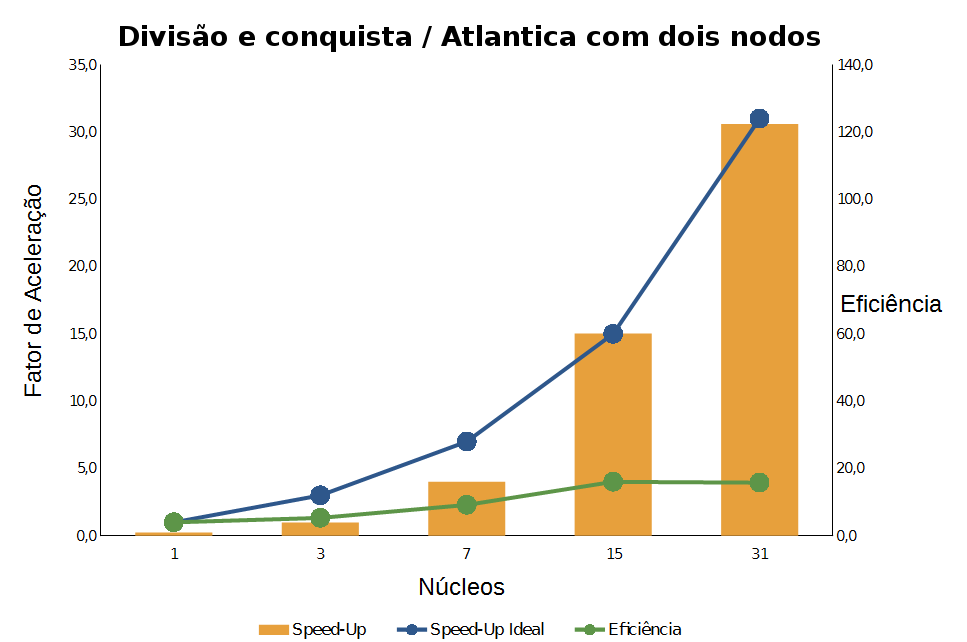
\includegraphics[width=\columnwidth]{fig/grafico.png}
\label{fig:grafico}
\end{Figure}
\section{Observações finais}
O que podemos concluir é que este problema possui um melhor desempenho quando utilizado em paralelo. Isto vem do fato de que o algoritmo do \textit{Bubble Sort} tem sua complexidade quadrática, e assim a medida que o problema vai sendo dividido entre mais processos, a carga de processamento em cada processo é muito menor, desta forma temos uma explosão de eficiência quando o problema é dividido. No final podemos ver que a eficiência se mantem a mesma para os dois últimos testes, mas o \textit{speedup} cresce, o que significa que o processamento se mantém o mesmo para a quantidade de processos disponíveis, ou seja, há ganho na velocidade de processamento por conta de ter mais processos, mas a eficiência continua igual.  

\end{multicols}

\newpage{}
\section{Código}

}
%{\scriptsize \tiny %LEO TESTA COM ESSE AQUI E VÊ QUE TU ACHA PORQUE DAI CABE EM UMA PAGINA
%\begin{verbatim}
\begin{lstlisting}
#include <stdio.h>
#include <stdlib.h>
#include "mpi.h"

#define DELTA 100000
#define VECTOR_INITIAL_SIZE 100000 

int *vetor;

void bs(int n, int * vetor){
	int c=0, d, troca, trocou =1;
	while (c < (n-1) & trocou ){
		trocou = 0;
		for (d = 0 ; d < n - c - 1; d++)
			if (vetor[d] > vetor[d+1]) {
				troca      = vetor[d];
				vetor[d]   = vetor[d+1];
				vetor[d+1] = troca;
				trocou = 1;
				}
		c++;
		}
}

int *interleaving(int vetor[], int tam){
	int *vetor_auxiliar;
	int i1, i2, i_aux;
	vetor_auxiliar = (int *)malloc(sizeof(int) * tam);
	i1 = 0;
	i2 = tam / 2;
	for (i_aux = 0; i_aux < tam; i_aux++) {
		if (((vetor[i1] <= vetor[i2]) && (i1 < (tam / 2)))
			|| (i2 == tam))
			vetor_auxiliar[i_aux] = vetor[i1++];
		else
			vetor_auxiliar[i_aux] = vetor[i2++];
	}
	return vetor_auxiliar;
}

int main(int argc, char** argv){
	int my_rank;           /* Identificador do processo */
	int proc_n;            /* Numero de processos */
	MPI_Status status;     /* Status de retorno */
	int vectorSize;        /* Tamanho do vetor recebido por tag */
	int filhoEsq, filhoDir, pai;

	MPI_Init (&argc, &argv);

	double t1,t2;
	t1 = MPI_Wtime();  // inicia a contagem do tempo

	MPI_Comm_rank(MPI_COMM_WORLD, &my_rank);
	MPI_Comm_size(MPI_COMM_WORLD, &proc_n);

	filhoEsq = my_rank*2 + 1;
	filhoDir = my_rank*2 + 2;

	if(my_rank!=0){
		//Recebe do pai
		MPI_Probe(MPI_ANY_SOURCE, MPI_ANY_TAG, MPI_COMM_WORLD, &status);
		vectorSize = status.MPI_TAG;
		pai = status.MPI_SOURCE;
		vetor = malloc(sizeof(int) * vectorSize);
		MPI_Recv (vetor, status.MPI_TAG, MPI_INT, pai, MPI_ANY_TAG, MPI_COMM_WORLD, &status);
	}else{
		//Gera vetor inicial
		vectorSize = VECTOR_INITIAL_SIZE;
		vetor = malloc(sizeof(int) * vectorSize);
		int i;
		for (i=0 ; i<vectorSize; i++){
			vetor[i] = vectorSize-i;
		}
	}

	if(vectorSize <= DELTA){
		//Conquista
		bs(vectorSize, vetor);
		int i = 0;
	}else{
		//Divide
		MPI_Send(&vetor[0], vectorSize/2, MPI_INT, filhoEsq, vectorSize/2, MPI_COMM_WORLD);
		MPI_Send(&vetor[vectorSize/2], vectorSize/2 + (vectorSize%2),
				 MPI_INT, filhoDir, vectorSize/2 + (vectorSize%2), MPI_COMM_WORLD);

		//Recebe
		MPI_Recv (&vetor[0], vectorSize/2, MPI_INT, filhoEsq, MPI_ANY_TAG, MPI_COMM_WORLD, &status);
		MPI_Recv (&vetor[vectorSize/2], vectorSize/2 + (vectorSize%2), 
				  MPI_INT, filhoDir, MPI_ANY_TAG, MPI_COMM_WORLD, &status);
		
		//Junta e manda para o pai
		vetor = interleaving(vetor, vectorSize);
	}
	
	if(my_rank!=0) {
		MPI_Send(vetor, vectorSize, MPI_INT, pai, 0, MPI_COMM_WORLD);
	}else{
		t2 = MPI_Wtime(); // termina a contagem do tempo
		printf("\nTempo de execucao: %f\n\n", t2-t1);   
	}
	
	MPI_Finalize();
}
\end{lstlisting}
%\end{verbatim}
%}
\end{document}
